\documentclass[aspectratio=169,11pt]{beamer}
\usepackage[T1]{fontenc}
\usepackage{lmodern,amsmath,amssymb,mathtools,bm,booktabs,array,graphicx,tikz}
\usetikzlibrary{arrows.meta,positioning,calc,decorations.pathreplacing,patterns}
\definecolor{ink}{HTML}{17344D}\definecolor{accent}{HTML}{087E8B}\definecolor{pale}{HTML}{EDF5F5}\definecolor{gold}{HTML}{AD6B19}
\providecommand{\dd}{\,\mathrm{d}}\providecommand{\R}{\mathbb{R}}
\providecommand{\E}{\mathbb{E}}\providecommand{\Var}{\operatorname{Var}}
\providecommand{\Cov}{\operatorname{Cov}}\providecommand{\diag}{\operatorname{diag}}
\providecommand{\norm}[1]{\left\lVert#1\right\rVert}
\providecommand{\abs}[1]{\left|#1\right|}
\usefonttheme{professionalfonts}
\setbeamercolor{normal text}{fg=black,bg=white}
\setbeamercolor{frametitle}{fg=ink,bg=white}
\setbeamercolor{title}{fg=ink}\setbeamercolor{structure}{fg=accent}
\setbeamercolor{block title}{fg=ink,bg=pale}\setbeamercolor{block body}{fg=black,bg=pale!40}
\setbeamercolor{alerted text}{fg=accent}
\setbeamerfont{frametitle}{size=\Large,series=\bfseries}
\setbeamerfont{title}{size=\LARGE,series=\bfseries}
\setbeamertemplate{navigation symbols}{}
\setbeamersize{text margin left=.7cm,text margin right=.7cm}
\setbeamertemplate{frametitle}{\vspace{.18cm}\insertframetitle\par\vspace{.1cm}{\color{accent}\hrule height .6pt}\vspace{.12cm}}
\newcommand{\notestarget}{notes.pdf}\newcommand{\noteslabel}{Notes}
\setbeamertemplate{footline}{\hspace{.7cm}\color{ink}\scriptsize Mathematical Cardiology\quad\href{\notestarget}{\noteslabel}\hfill\insertframenumber\,/\,\inserttotalframenumber\hspace{.7cm}\vspace{.18cm}}
\setbeamercovered{invisible}
\hypersetup{pdfauthor={Zan Ahmad},pdftitle={From image geometry to a tracer balance},pdfpagemode=UseNone}
\begin{document}
\begin{frame}[plain]\vfill
{\small\color{accent} Mathematical Cardiology \quad Lecture 9}\par\medskip
{\raggedright\hyphenpenalty=10000\exhyphenpenalty=10000\LARGE\bfseries\color{ink} From image geometry to a tracer balance}\par\bigskip
Zan Ahmad\par\smallskip
{\small Fall 2023}\par\vfill\end{frame}
\renewcommand{\notestarget}{notes.pdf\#note-an-intensity-field-and-a-selected-region}
\begin{frame}[label=slide-a-picture-contains-intensities-figure]{A picture contains intensities}
\centering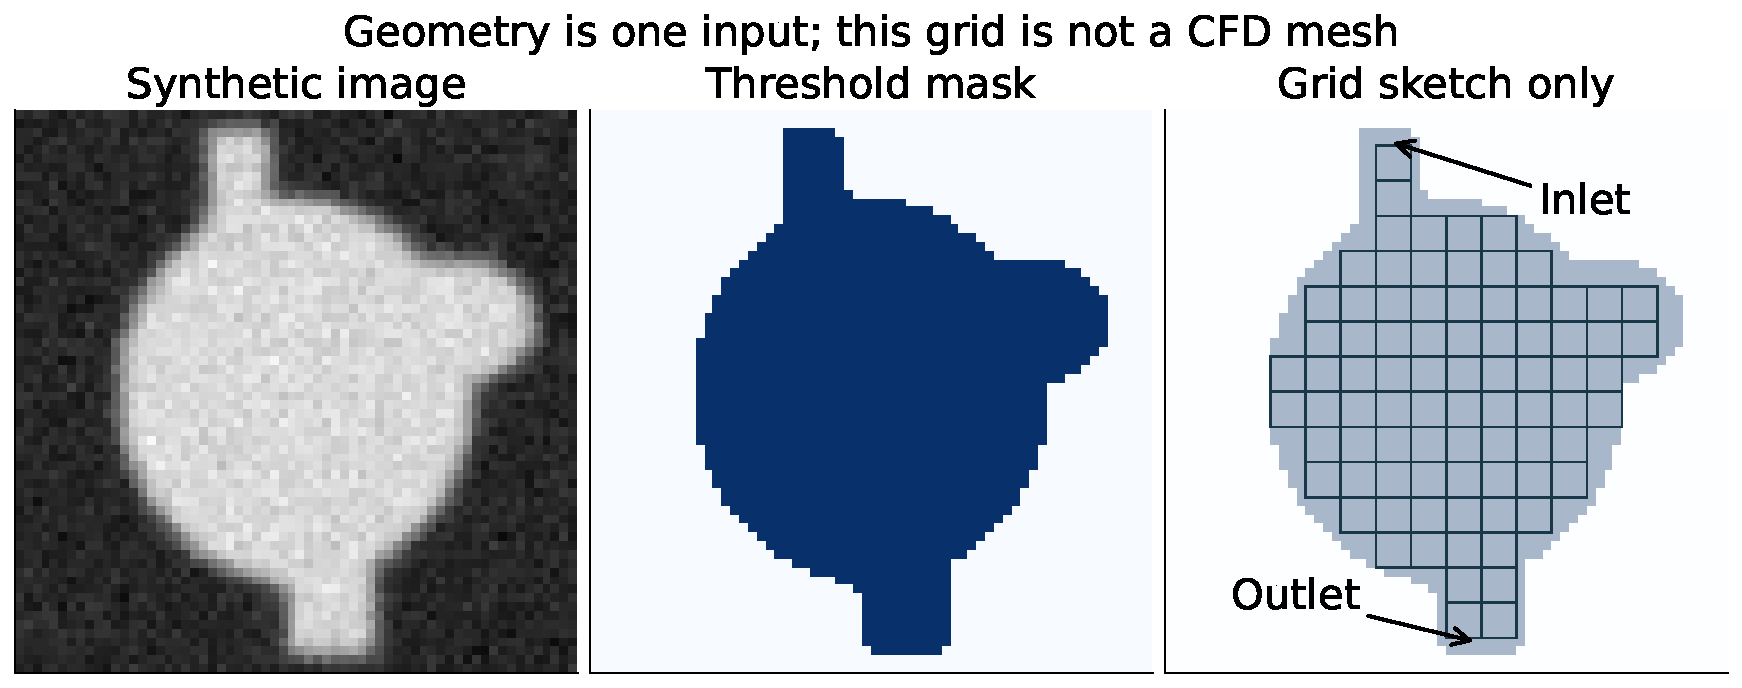
\includegraphics[width=.98\linewidth,height=.69\textheight,keepaspectratio]{image-pipeline.pdf}\end{frame}
\renewcommand{\notestarget}{notes.pdf\#note-an-intensity-field-and-a-selected-region}
\begin{frame}[t,fragile,label=slide-a-picture-contains-intensities]{A picture contains intensities}
\[I=(I_{ij}),\qquad M_{ij}(\theta)=\mathbf1\{I_{ij}\geq\theta\}.\]
\pause{}
The image, the mask and the computational region are different objects.
\end{frame}
\renewcommand{\notestarget}{notes.pdf\#note-an-intensity-field-and-a-selected-region}
\begin{frame}[t,fragile,label=slide-increasing-a-threshold-selects-a-subset]{Increasing a threshold selects a subset}
If $\theta_2>\theta_1$,
\[I_{ij}\geq\theta_2\Longrightarrow I_{ij}\geq\theta_1.\]
\pause{}
Thus $N(\theta_2)\leq N(\theta_1)$.
\[1699\geq1641\geq1563\quad\text{at }0.4,0.5,0.6.\]
\end{frame}
\renewcommand{\notestarget}{notes.pdf\#note-an-intensity-field-and-a-selected-region}
\begin{frame}[t,fragile,label=slide-pixel-count-needs-a-physical-scale]{Pixel count needs a physical scale}
For spacings $s_x,s_y$,
\[A=N s_xs_y.\]
\pause{}
Changing a pixel count does not determine a volume.
Out-of-plane geometry is missing from a single two-dimensional mask.
\end{frame}
\renewcommand{\notestarget}{notes.pdf\#note-connectivity-and-the-missing-spatial-problem}
\begin{frame}[t,fragile,label=slide-a-small-area-change-can-alter-a-route]{A small area change can alter a route}
A narrow neck may contain few pixels.
\pause{}
Removing those pixels can disconnect the pocket while changing total area only slightly.

Inspect the neck, top inlet, lower outlet and remaining wall boundary.
\end{frame}
\renewcommand{\notestarget}{notes.pdf\#note-connectivity-and-the-missing-spatial-problem}
\begin{frame}[t,fragile,label=slide-conservation-on-each-cell]{Conservation on each cell}
With outward volume flux positive,
\[\sum_{f\in\partial\mathrm{cell}}Q_f=0.\]
\pause{}
At a shared face, one cell's outward flow is the other's inward flow.
Internal fluxes cancel when cells are added.
\end{frame}
\renewcommand{\notestarget}{notes.pdf\#note-connectivity-and-the-missing-spatial-problem}
\begin{frame}[t,fragile,label=slide-the-spatial-problem-needs-more-information]{The spatial problem needs more information}
The top opening needs an inlet condition; the lower opening needs an outlet condition.
\pause{}
Walls, fluid properties and momentum balance determine how a velocity field can develop.
A mesh supplies locations for the calculation, not these laws.
\end{frame}
\renewcommand{\notestarget}{notes.pdf\#note-a-deliberately-well-mixed-reduction}
\begin{frame}[t,fragile,label=slide-reduce-the-region-to-one-mixed-volume]{Reduce the region to one mixed volume}
\[M=VC.\]
$M$ is tracer amount and $C$ is tracer amount per fluid volume.
\pause{}
Equal inflow and outflow $Q$ keep $V$ fixed.
Complete mixing makes outlet concentration equal to $C$.
\end{frame}
\renewcommand{\notestarget}{notes.pdf\#note-a-deliberately-well-mixed-reduction}
\begin{frame}[t,fragile,label=slide-balance-the-tracer-over-a-short-interval]{Balance the tracer over a short interval}
\[M(t+h)-M(t)\simeq hQ C_{\rm in}-hQC(t).\]
\pause{}
For tracer-free inflow,
\[C_{n+1}=(1-hQ/V)C_n.\]
\end{frame}
\renewcommand{\notestarget}{notes.pdf\#note-a-deliberately-well-mixed-reduction}
\begin{frame}[t,fragile,label=slide-a-time-step-condition]{A time-step condition}
For $C_n\geq0$, the explicit update stays nonnegative if
\[0\leq hQ/V\leq1.\]
\pause{}
A larger step can create a negative numerical concentration.
The companion uses the exact exponential, not this update.
\end{frame}
\renewcommand{\notestarget}{notes.pdf\#note-the-exponential-and-its-time-scale}
\begin{frame}[t,fragile,label=slide-repeated-removal-gives-an-exponential]{Repeated removal gives an exponential}
Use $n$ steps over time $t$:
\[C_n/C_0=(1-Qt/(nV))^n.\]
\pause{}
As the steps become finer,
\[\boxed{C(t)/C_0=e^{-Qt/V}}.\]
\end{frame}
\renewcommand{\notestarget}{notes.pdf\#note-the-exponential-and-its-time-scale}
\begin{frame}[label=slide-the-time-constant-is-a-volume-to-flow-ratio-figure]{The time constant is a volume-to-flow ratio}
\centering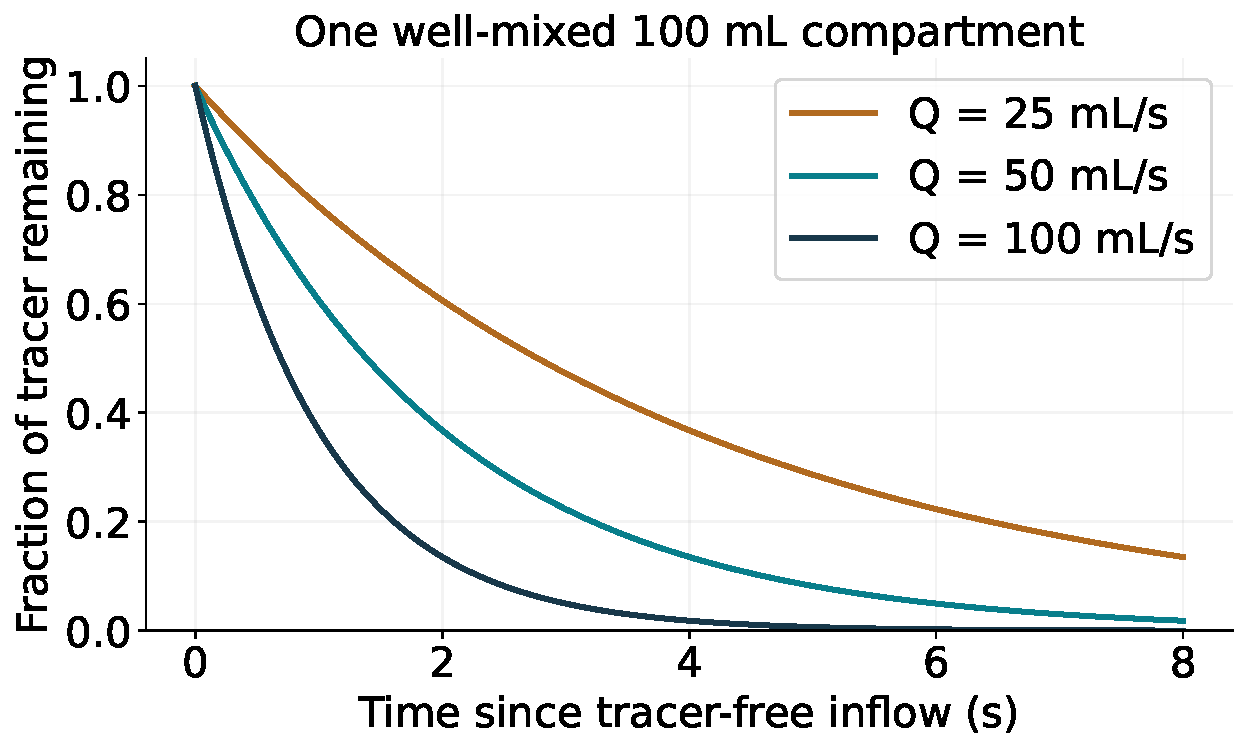
\includegraphics[width=.98\linewidth,height=.69\textheight,keepaspectratio]{washout.pdf}\end{frame}
\renewcommand{\notestarget}{notes.pdf\#note-the-exponential-and-its-time-scale}
\begin{frame}[t,fragile,label=slide-the-time-constant-is-a-volume-to-flow-ratio]{The time constant is a volume-to-flow ratio}
\[\tau=V/Q,\qquad C(t)/C_0=e^{-t/\tau}.\]
\pause{}
At $t=\tau$, the remaining fraction is $e^{-1}\simeq0.368$.
At half-time, $t_{1/2}=\tau\log2$.
\end{frame}
\renewcommand{\notestarget}{notes.pdf\#note-the-exponential-and-its-time-scale}
\begin{frame}[t,fragile,label=slide-evaluate-the-three-curves]{Evaluate the three curves}
At $V=100\,\mathrm{mL}$ and $t=2\,\mathrm{s}$,
\[
\begin{array}{c|rrr}
Q\ (\mathrm{mL/s})&25&50&100\\\hline
\tau\ (\mathrm{s})&4&2&1\\
C/C_0&0.607&0.368&0.135
\end{array}
\]
\end{frame}
\renewcommand{\notestarget}{notes.pdf\#note-the-exponential-and-its-time-scale}
\begin{frame}[t,fragile,label=slide-an-identifiability-limitation]{An identifiability limitation}
For any $a>0$,
\[\frac{aQ}{aV}=\frac QV.\]
\pause{}
The decay curve cannot distinguish $(V,Q)$ from $(aV,aQ)$.
If $Q=0$, concentration remains constant.
\end{frame}
\renewcommand{\notestarget}{notes.pdf\#note-a-separate-concentration-state-for-the-pocket}
\begin{frame}[t,fragile,label=slide-a-pocket-needs-its-own-state]{A pocket needs its own state}
An optional two-compartment extension is
\[V_a\dot C_a=-QC_a+q(C_b-C_a),\]
\[V_b\dot C_b=q(C_a-C_b).\]
\pause{}
The companion does not solve these equations.
\end{frame}
\renewcommand{\notestarget}{notes.pdf\#note-a-separate-concentration-state-for-the-pocket}
\begin{frame}[t,fragile,label=slide-add-the-two-balances]{Add the two balances}
\[\frac{\mathrm d}{\mathrm dt}(V_aC_a+V_bC_b)=-QC_a.\]
Internal exchange cancels.
\pause{}
If $q=0$, tracer initially in the pocket remains there.
One mixed concentration cannot represent this case.
\end{frame}
\renewcommand{\notestarget}{notes.pdf\#note-numerical-refinement-and-independent-validation}
\begin{frame}[t,fragile,label=slide-two-different-tests]{Two different tests}
Keep physics fixed and refine mesh and time step:
compare a named output for numerical sensitivity.
\pause{}
Compare that output with independent measurements:
test the physical model.

Neither comparison alone turns washout into a stroke prediction.
\end{frame}
\end{document}
